\documentclass{deliverablereport}

\usepackage[style=alphabetic,backend=bibtex]{biblatex}
\addbibresource{report.bib}
\addbibresource{../../lib/publications.bib}

\usepackage{xparse}
\usepackage{etoolbox}
\usepackage{caption}
\graphicspath{{events/}}
 \ExplSyntaxOn

\newcounter{eventcounter}

\newenvironment{event}[7]{
\vspace{0.5cm}
\refstepcounter{eventcounter}
\label{event-#2}


\noindent\textbf{Event~\theeventcounter -~ #1}\newline % title

\noindent #3 \newline % location and date

\noindent ODK~partners~involved:~ \clist_map_inline:nn{#4}{\site{##1}~}\newline %partners

\ifx&#5&%
      % no participant #
\else
\noindent #5~participants~
\ifx&#6 &%
    % no odk participant
\else 
~(including~#6~from~within~ODK)\newline
\fi
\fi

\ifx&#7&%
      % no website
\else
\noindent \url{#7}\newline
\fi



}{\begin{center}\noindent\rule{4cm}{0.4pt}\end{center}}

 \ExplSyntaxOff


\deliverable{dissem}{workshops-3}
\duedate{31/08/2018 (M36)}
\deliverydate{31/08/2018}
\author{Viviane Pons et al.}

\begin{document}
\enlargethispage{4ex}
\maketitle
\githubissuedescription
\tableofcontents
\newpage

% Other tasks and deliv impacted: T3.6, T4.1, T6.1, T6.3, T6.10, D6.2 WP5 D4.4 D4.7 T3.1 T4.4 T4.6

\section{Project meetings and development workshops}

We call a development workshop an event with a restricted number of participants
who meet to work on a specific task. These workshops are an inherent part
of \ODK development process as described in \taskref{dissem}{devel-workshops}:
 they bring together
developers from within and outside of \ODK and allow effective work
and discussions on many technical aspects. They also participate in building
and maintaining a community of developers inside \ODK and within the
open-source communities we belong to.

We list here all workshops which have been organized or co-organized by \ODK
as well as external workshops which have been attended by \ODK participants
with a significant impact on the project. We also include project meetings as they
participate to the same goal of bringing together participants of the project and
always include some development time.

Throughout year 2 and 3 of the project, we have had

%TODO : replace XXX in budget
\begin{event}{Atelier PARI/GP 2017}{AtelierPARI2017}{Grenoble (FR),
2017-01-09 to 2017-01-13}{PS,UB,UV,UW}{36}{http://pari.math.u-bordeaux.fr/Events/PARI2017/}

\textbf{Main goals.}

The PARI/GP Ateliers were established in 2012 as a yearly meeting
between developers and users of the PARI/GP system.

The main goals are advertising new features and improvements,
discussing further developments, sharing best practices, and collaborative
code writing (hacking sessions, doc reviews, bug-squashing parties).

You can find the list of previous PARI Ateliers at
\url{http://pari.math.u-bordeaux.fr/ateliers.html}

\textbf{ODK implication.} 
%Describe how ODK was involved and give a rough estimation of cost for ODK

\ODK participants: B. Allombert, K. Belabas, V. Delecroix, J. Demeyer,
J.-P. Flori, L. de Feo.

\ODK provided the main funding source for the workshop (accommodation,
subsistence and travel expenses), for about XXXk\euro. The Lyon
institute of mathematics (Institut Camille Jordan) co-funded the event.

\textbf{Event summary.} 
%Give a summary of your event

The 7th Atelier PARI/GP took place in Lyon (France) from january
9th to 13th.

There were 43 registered participants from 19 different institutions
(no registration fees).

A typical day of the workshop had introductory talks and tutorials
in the morning; afternoons allowed ample time for hacking sessions,
discussions and training.

The Atelier featured 10 morning talks on mathematical topics and
implementation projects including 4 talks by ODK members
\begin{itemize}
\item Karim Belabas ``Using GIT with PARI'', ``$L$-functions'' and
  ``Dirichlet characters''
\item Bill Allombert ``New GP features''
\end{itemize}

Slides for all talks are available at
\url{http://pari.math.u-bordeaux.fr/Events/PARI2017/}

\textbf{Results and impact.} 
% What did you achieve with this event? (If ever it impacted 
% other ODK tasks and deliverables, mention it here)

The workshop was very productive and particularly beneficial to WP5
(high-performance computing). It also was a successful dissemination event: half
  the participants had not come to a previous Atelier.

\end{event}


%TODO : replace XXX in budget
\begin{event}{Atelier PARI/GP 2017b}{AtelierPARI2017b}{Clermont-Ferrand (FR),
2017-06-19 to 2017-06-23}{PS,UB,UV,UW}{36}{3}{http://pari.math.u-bordeaux.fr/Events/PARI2017b/}


\textbf{ODK implication.} 
%Describe how ODK was involved and give a rough estimation of cost for ODK

\ODK participants: B. Allombert, K. Belabas, J.-P. Flori

\ODK provided the main funding source for the workshop (accommodation,
subsistence and travel expenses), for about 12k\euro. The following
institutions co-funded the event through Clermont institute of mathematics
  (Laboratoire
  Blaise Pascal): GDR Structuration de la Théorie des Nombres (CNRS), Région
  Auvergne Rhône-Alpes, Conseil départemental Puy-de-Dôme, Université
  Auvergne-Rhônes-Alpes and the city of Clermont-Ferrand.

\textbf{Event summary.} 
%Give a summary of your event

The 8th Atelier PARI/GP took place in Clermont-Ferrand (France) from june
19th to 23rd with a special focus on Elliptic curves, Modular Forms and
$L$-Functions.

There were 36 registered participants from 16 different institutions
(no registration fees).

A typical day of the workshop had introductory talks and tutorials
in the morning; afternoons allowed ample time for hacking sessions,
discussions and training.

The Atelier featured 13 morning talks.

\textbf{Results and impact.} 
% What did you achieve with this event? (If ever it impacted 
% other ODK tasks and deliverables, mention it here)
This was a dissemination event with a special focus on recently developped
packages (Elliptic curves over number fields, Modular forms), before they were
merged into a formal release. We got lots of feedback on the interface and
documentation and a number of bugs and glitches were fixed as a result.
\end{event}


%TODO complete
\begin{event}{Project meeting in XFEL}{PMxfel}{XFEL Hamburg, June 20 --22, 2018}{XFEL, PS, LL, UW, LEEDS, SR, US, UK}{13}{13}{https://opendreamkit.org/2018/06/20/Hamburg-DisseminationWorkshop-SteeringMeeting/}

\textbf{Main goals.} At the occasion of the project meeting, we also held a workshop on dissemination and a Jupyter workshop on 3d graphics.

\textbf{ODK implication.} The event was hosted by XFEL and each participant was funded by ODK through their institutions.

\textbf{Event summary.} The first part of the event was focused on dissemination and communication in ODK. It was an occasion to expose what had been done in the previous years and start a reflexion on how to better promote it. We discussed the new website design and organization and we wrote some new content. We also had a professional interviewer on site who conducted interviews of the ODK team to give an overview of the project goals, accomplishments, and philosophy. The second part of the event was dedicated to a Jupyter workshop on 3d graphics.

\textbf{Demographic.} All participants were ODK members.

\textbf{Results and impact.} This was a very useful consultation. The new website was released in the following weeks. The interviews are still being edited but should be live soon.


\end{event}


\section{Dissemination and outreaching activities}

We describe here all activities related to \taskref{dissem}{dissemination}:
these are all events oriented towards dissemination, training, and outreach. This
includes events organized or co-organized by \ODK and also
participating in external events and many communication activities.

\subsection{Training workshops}

\begin{event}{IOP Magnetism 2017 - Computational micromagnetics with JOOMMF workshop}{IOP2017}{University of York, UK, 04 April 2017}{XFEL}{30}{3}{http://magnetism2017.iopconfs.org/OOMMF}

\textbf{Main goals.} We introduced the basics of micromagnetics as well as taught the participants how to run OOMMF simulations using our Python interface - JOOMMF.

\textbf{ODK implication.} JOOMMF was developed as a part of the ODK project and three participants from the ODK were present to deliver the workshop (Hans Fangohr, Marijan Beg, and Ryan A. Pepper). The workshop was co-funded by the conference organisers and the EPSRC CCP Computational Magnetism Network (EP/M022668/1) grant. No costs of the workshop were paid from the ODK funds.

\textbf{Event summary.} In this workshop we provided a brief introduction to computational micromagnetics, Python, and the Jupyter notebook. We taught participants to use our Python interface to drive OOMMF micromagnetic simulation by guiding them through tutorials. At the beginning of the workshop, we provided a lecture style introduction, which was followed by practical exercises where attendees had an opportunity to carry out small micromagnetic calculations, modify given examples and ask more specific questions. This workshop was held together with Michael Donahue, NIST - one of the main developers of the OOMMF package.

\textbf{Demographic.} We had about 30 participants during the workshop, but due to the data protection regulations, the organisers did not allow us to have demographics information. During the workshop, 19 participants gave us their details with demographics: 13 males and 6 females.

\textbf{Results and impact.} During the workshop we received the feedback from the participants about our Python interface to OOMMF as well as gained experience which helped us to structure future workshops.

\end{event}


\begin{event}{Intermag 2017 - Computational micromagnetics with JOOMMF workshop}{Intermag2017}{Dublin, Ireland, 24 April 2017}{XFEL}{57}{2}{}

\textbf{Main goals.} We introduced the basics of computational micromagnetics as well as taught the participants how to run JOOMMF simulations.

\textbf{ODK implication.} JOOMMF was developed as a part of the ODK project and two participants from the ODK project were present to deliver the workshop (Marijan Beg, and Ryan A. Pepper). The workshop was co-funded by the conference organisers and the EPSRC CCP Computational Magnetism Network (EP/M022668/1) grant. No costs of the workshop were paid from the ODK funds.

\textbf{Event summary.} In this workshop we provided a brief introduction to computational micromagnetics. We introduced and taught the use of a Python interface to drive the OOMMF simulation package. At the beginning of the workshop, we provided a lecture style introduction, which was followed by practical exercises where attendees had an opportunity to carry out small micromagnetic calculations, modify given examples and ask more specific questions. Several days after the main event, we held a follow up session, where we were able to talk to participants about their specific needs, get requests for features, and get general feedback.

\textbf{Demographic.} We had 57 participants, but the organizers did not allow us to have their personal details.

\textbf{Results and impact.} During the workshop we received the feedback from the participants about our Python interface to OOMMF as well as gained experience which helped us to structure future workshops.

\begin{figure}[ht]
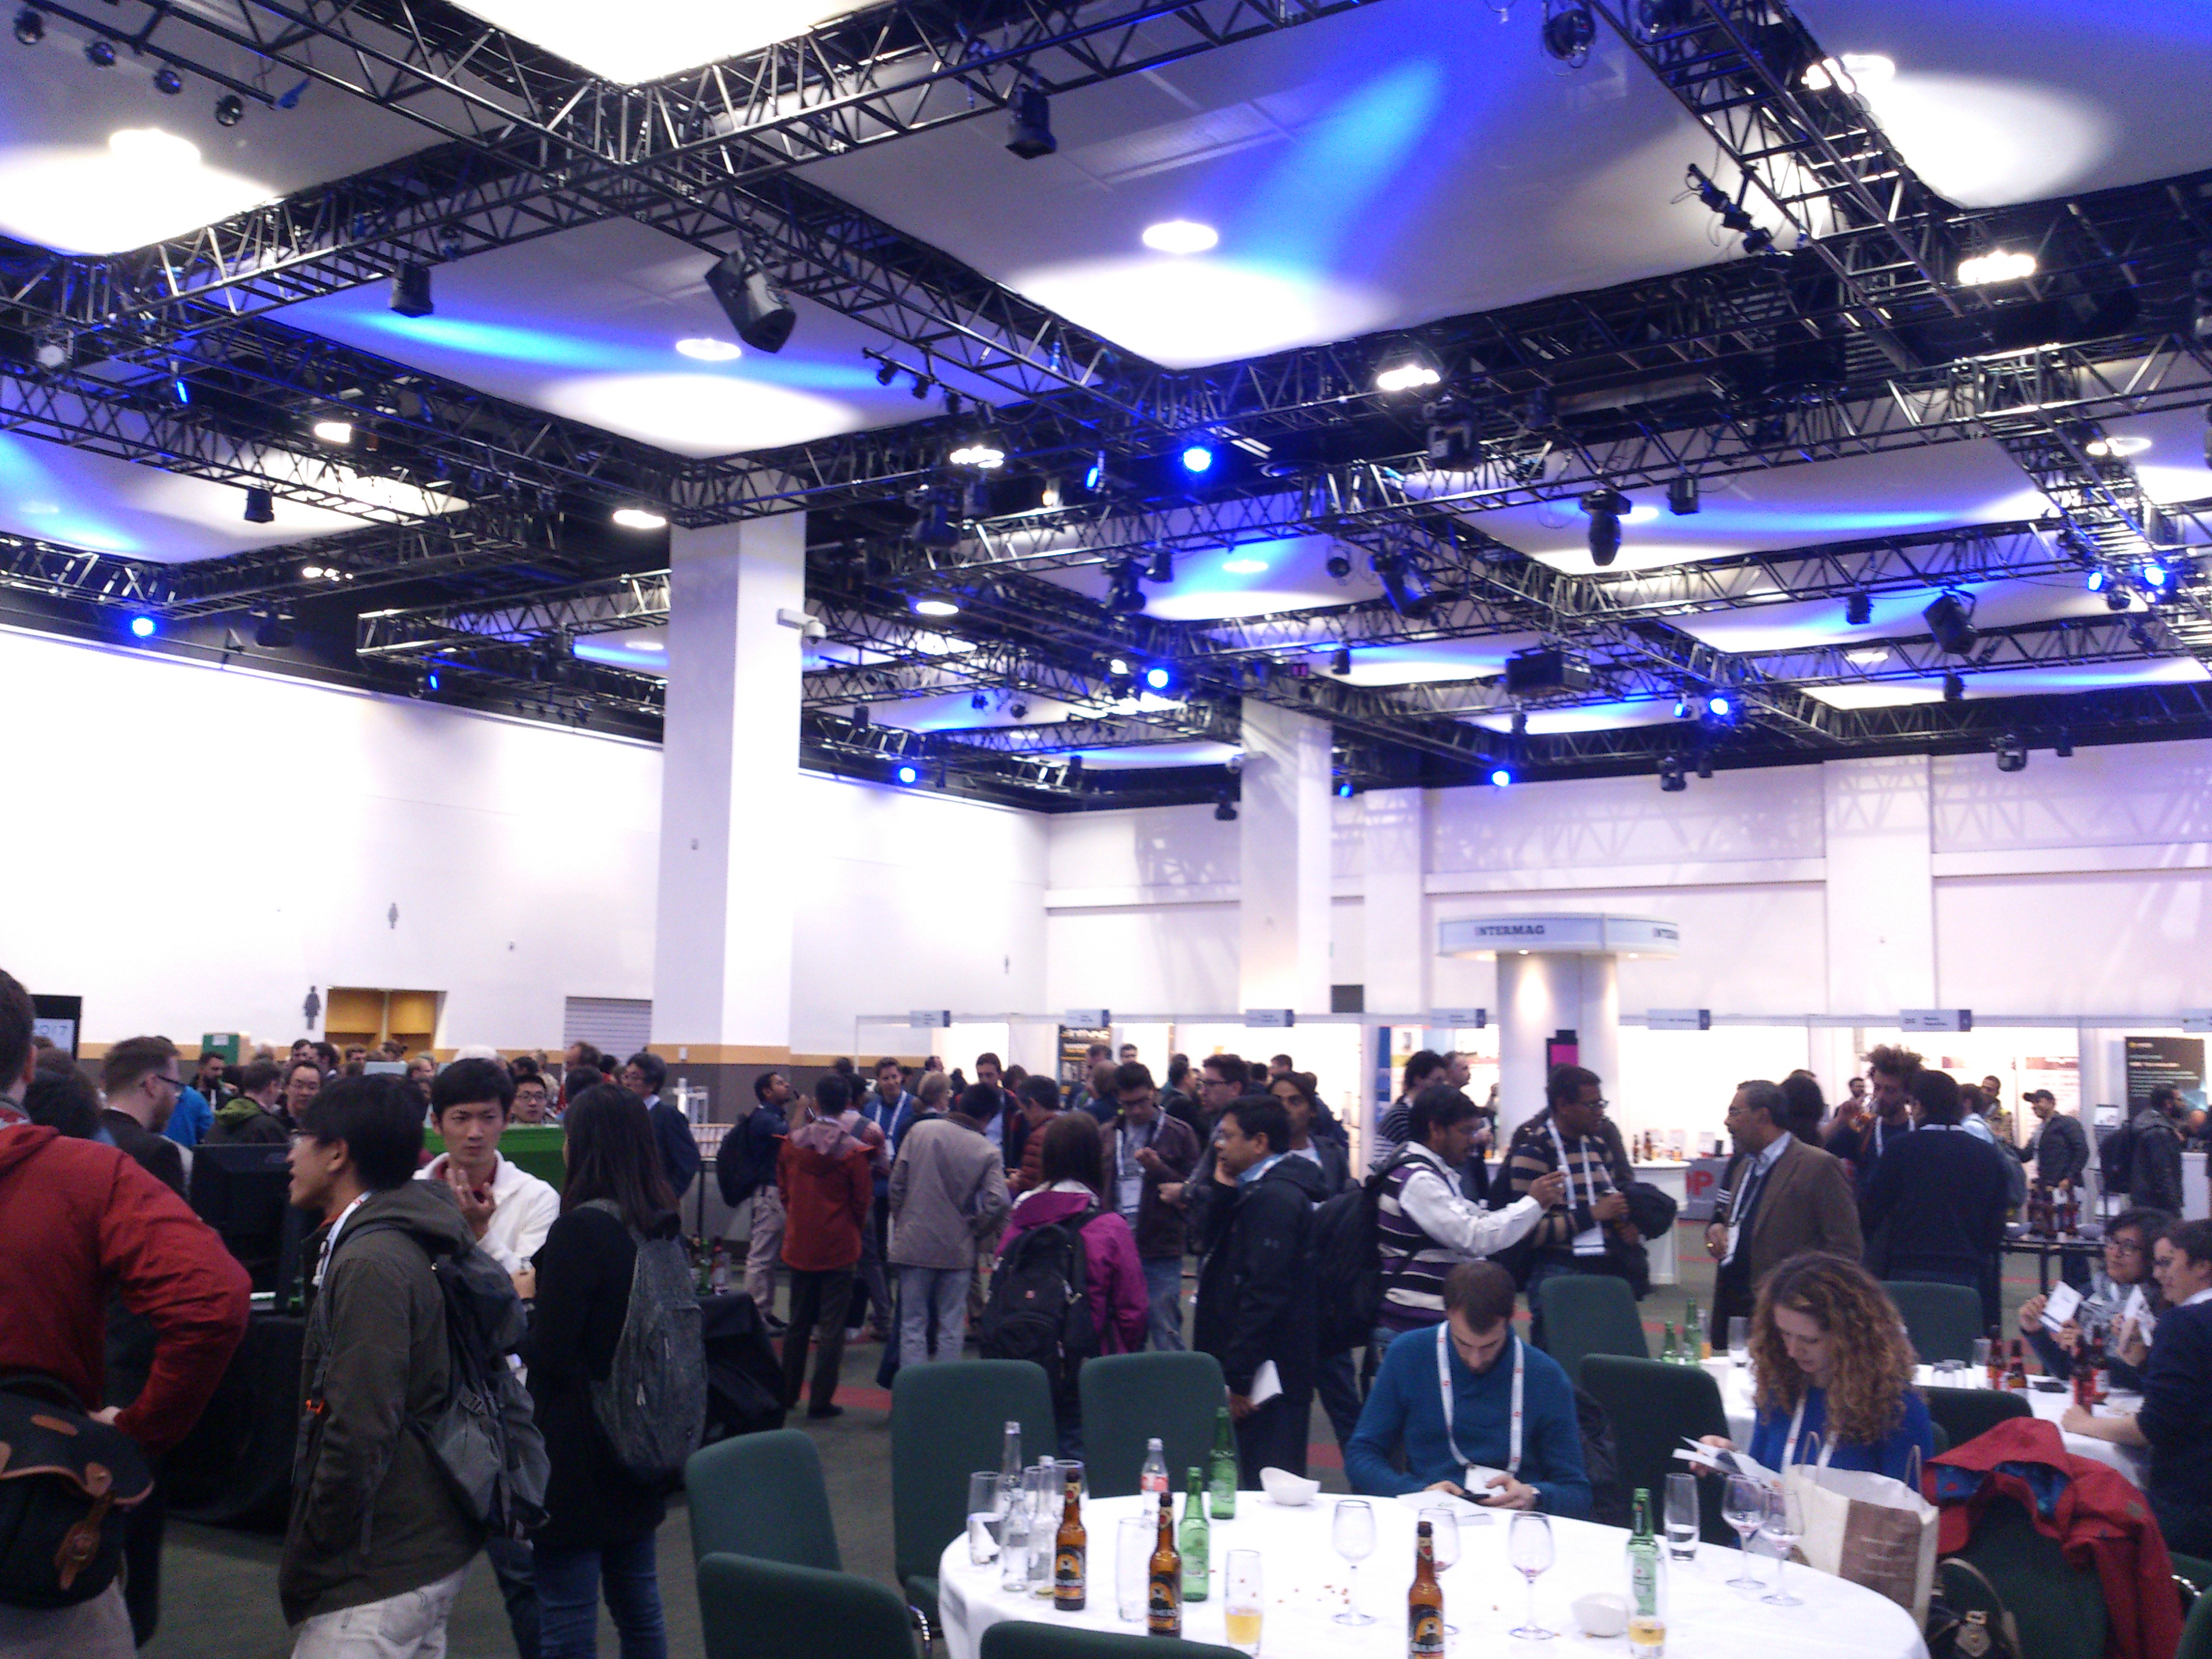
\includegraphics[scale=.1]{IntermagPhoto1.jpg}
\caption*{Intermag2017 conference in Dublin, Ireland.}
\end{figure}

\begin{figure}[ht]
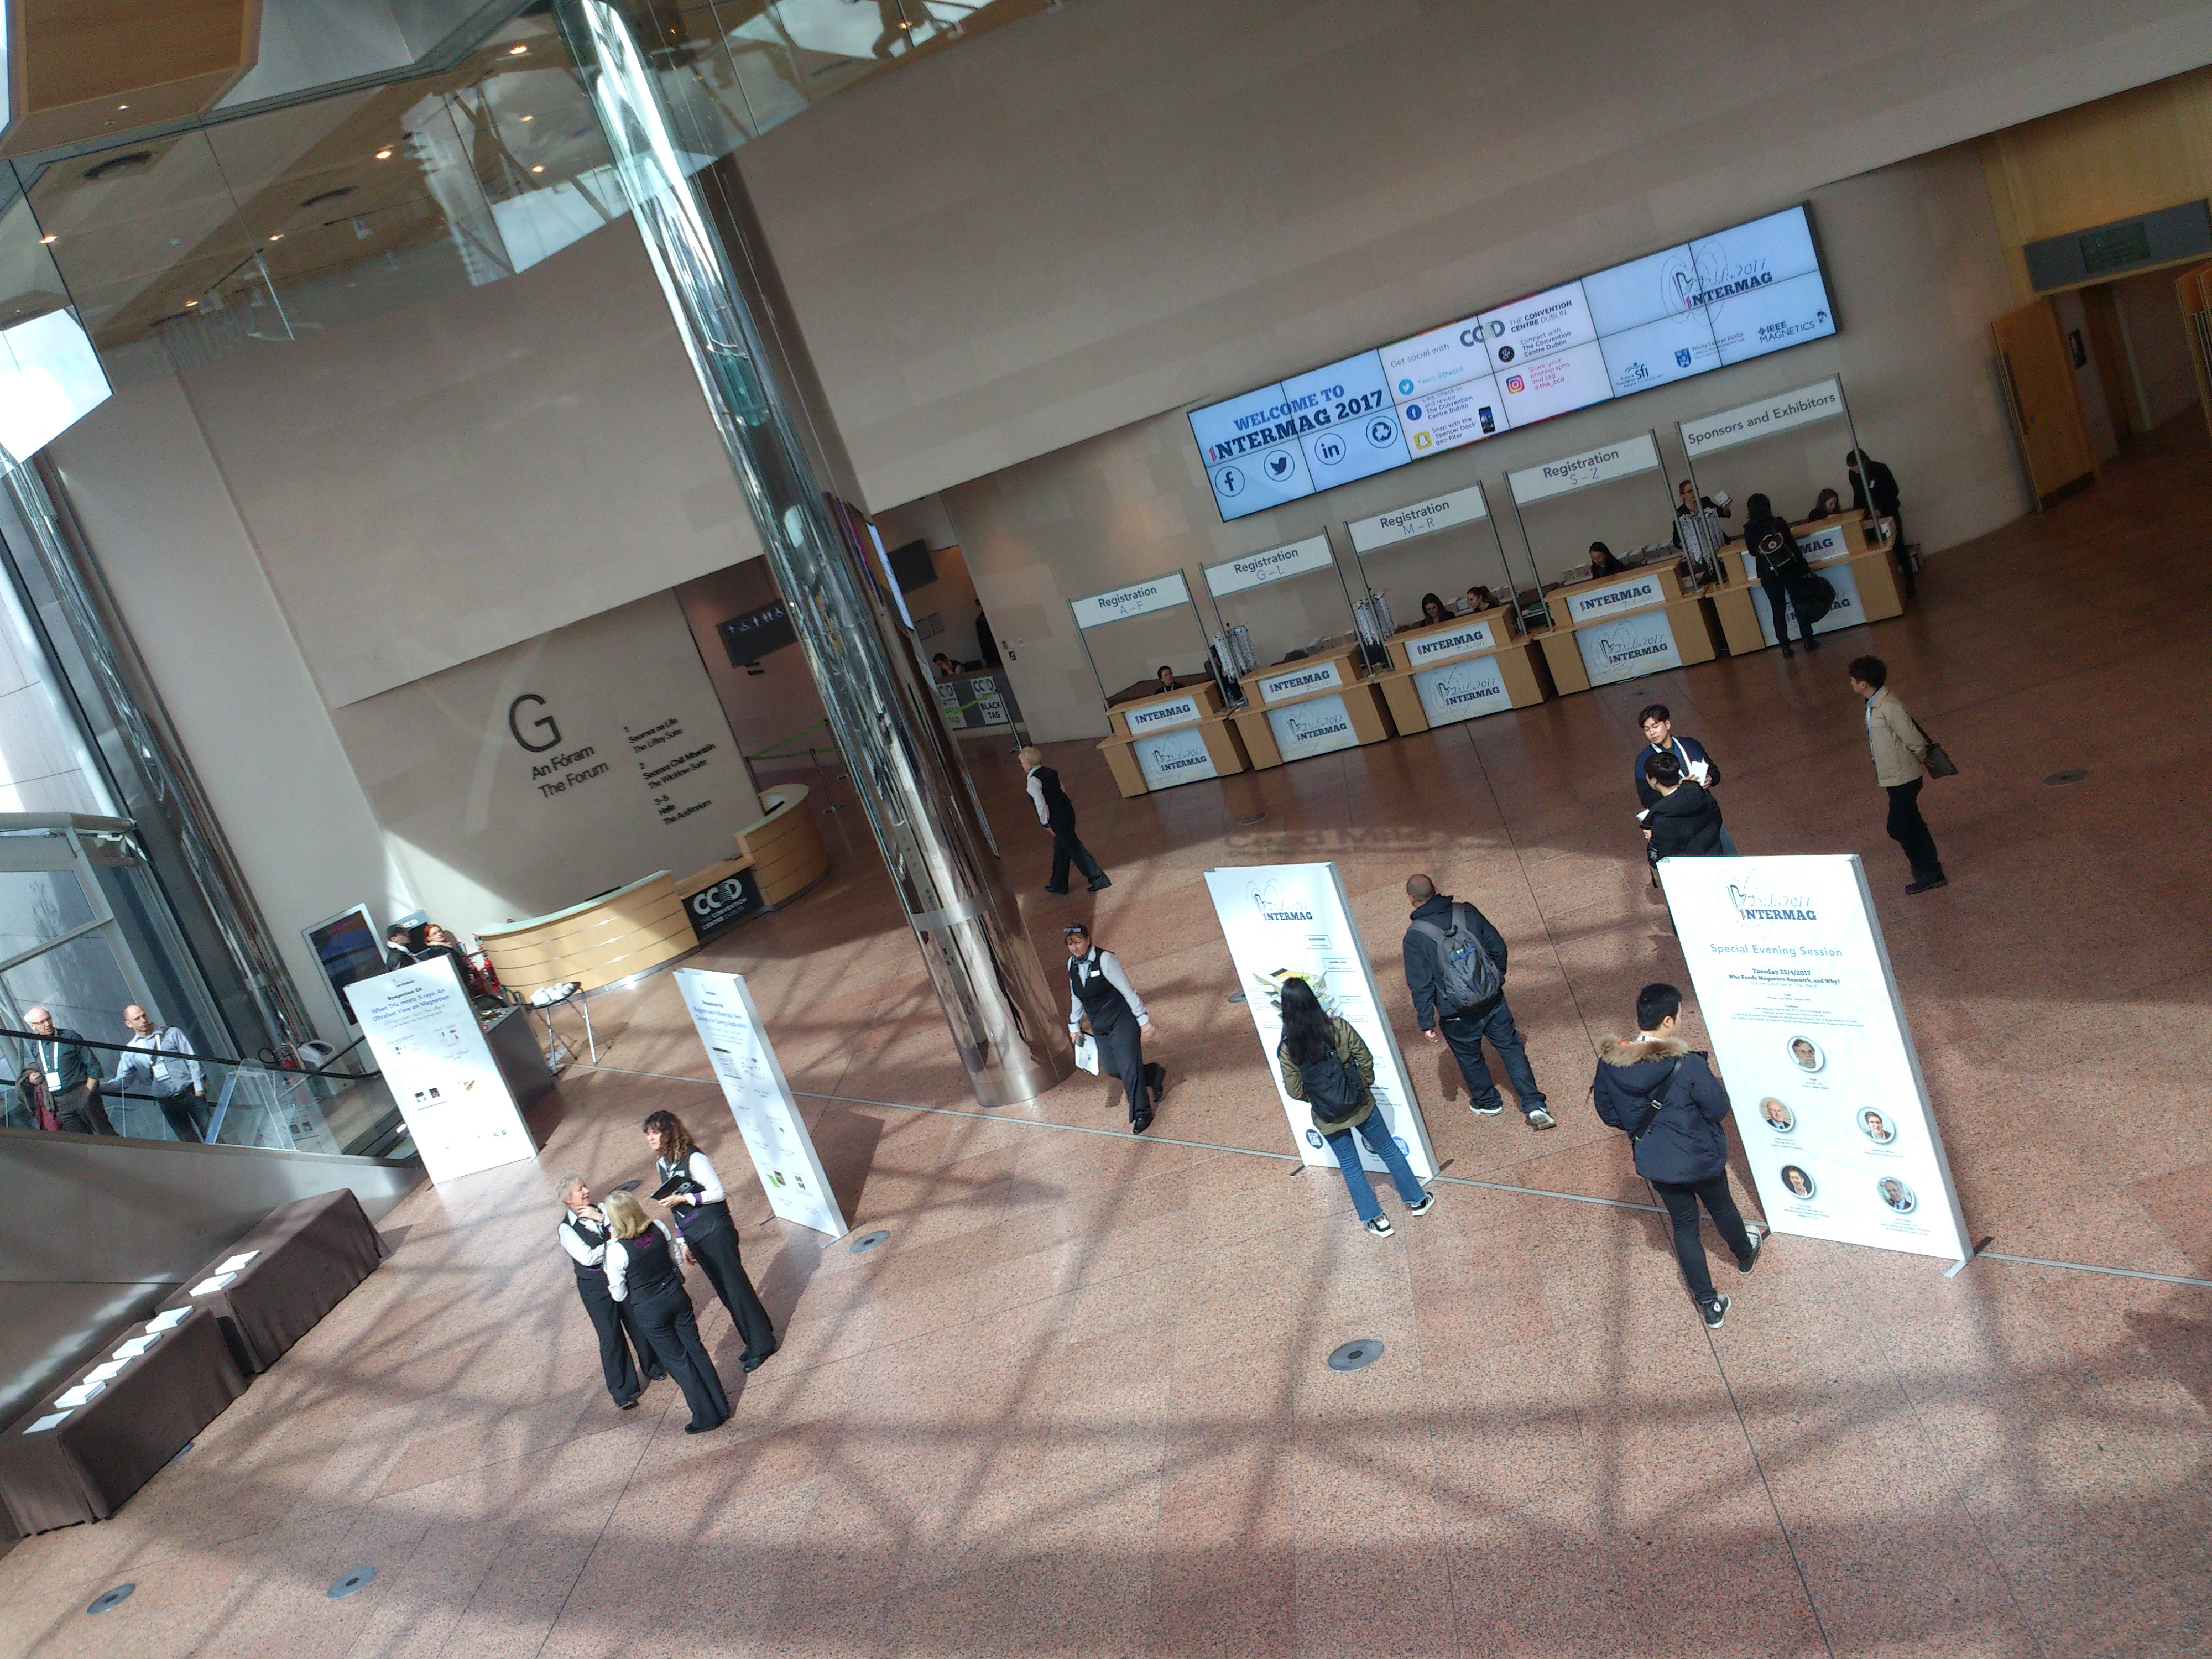
\includegraphics[scale=.1]{IntermagPhoto2.jpg}
\caption*{Intermag2017 conference in Dublin, Ireland.}
\end{figure}

\end{event}


\begin{event}{MMM 2017 - JOOMMF drop-in sessions}{MMM2017}{Pittsburgh, PA, USA 06-10 November 2017}{XFEL}{5}{1}{}

\textbf{Main goals.} In two sessions during the conference, users had a chance to talk to us, give us feedback, and request features.

\textbf{ODK implication.} JOOMMF was developed as a part of the ODK project and one participant from the ODK was present to deliver the workshop (Marijan Beg). The workshop was fully funded by the ODK and total costs were 2048.67 euros.

\textbf{Event summary.} In two drop-in sessions, we helped users with installation, looked at their simulation requirements, and received some feedback and feature requests.

\textbf{Results and impact.} During the workshop we received the feedback from the participants about our Python interface to OOMMF.

\end{event}


\begin{event}{Advances in Magnetism 2018 - Computational micromagnetics with JOOMMF tutorial}{AIM2018}{La Thuile, Italy, 04-07 Fabruary 2018}{XFEL}{100}{1}{No url.}

\textbf{Main goals.} We gave a tutorial about computational micromagnetics and JOOMMF to all conference participants.

\textbf{ODK implication.} JOOMMF was developed as a part of the ODK project and one participant from the ODK was present to deliver the tutorial (Marijan Beg). The tutorial was fully funded from the ODK funds and the total costs were 1207.73 euros.

\textbf{Event summary.} This tutorial was in the official part of the conference programme available to all atendees. We had about 100 participants and we introduced to them the basics of computational micromagnetics as well as gave them an introduction to JOOMMF. At the end, we answered any specific question attendees had.

\textbf{Demographic.} We had around 100 participants, but the organisers did not allow us to have their personal details due to the data protection.

\textbf{Results and impact.} We informed the community of potential users about the benefits of JOOMMF and provided to them enough information if they want to start using it.

\end{event}


\begin{event}{Atelier et \'Ecole MathExp 2018}{MathExp2018}{Saint-Flour (FR),
2018-05-21 to 2018-06-01}{UB}{36}{3}{https://mathexp2018.sciencesconf.org/}

\textbf{Main goals.}

The MathExp school and atelier organized in Saint Flour was a unique
opportunity for young mathematicians to learn about computer science
and the tools developed in the framework of \ODK. The event
was divided in two weeks. The first one focused on 4 courses and
introductory tutorials with SageMath and Jupyter. During the second
week the participants were asked to develop programs related to their
own research projects.

\textbf{ODK implication.} 
%Describe how ODK was involved and give a rough estimation of cost for ODK

\ODK organizer: V. Delecroix

\ODK provided the main funding source for the workshop (accommodation,
subsistence and some of the travel expenses) for about 40K\euro. There were
also inscription fees and the event was cofounded with the CNRS.

\textbf{Event summary.} 
%Give a summary of your event

The school and atelier MathExp took place in Saint-Flour (France)
from May 21st to June 1st.

There were 22 registered participants.

A typical day of the school consisted of 2 courses and tutorials
on computers. During the atelier, participants worked on their
own research projects asking for help when needed.

The School featured 4 courses on computer science topics directly
related to mathematical computations: probability (Ana Bušić (Paris, FR)),
linear programming (Xavier Goaoc (Marne-la-Vallée, FR)), formal computation
(Bruno Salvy (Lyon, FR)) and backtracking techniques (Michaël Rao (Lyon, FR)).

\textbf{Results and impact.} 
% What did you achieve with this event? (If ever it impacted 
% other ODK tasks and deliverables, mention it here)

We were delighted to achieve a gender equidistribution among the participants
(10 female and 12 males) which is not often in Mathematics and Computer
Science.

The school and workshop were very productive and beneficial to disseminate
the work achieved in the various work packages. In particular
all the work around SageMath and Jupyter.

\end{event}


\begin{event}{ICM 2018 - Computational micromagnetics with JOOMMF workshop}{ICM2018}{San Francisco, CA, USA, 15-20 July 2018}{XFEL}{130}{2}{No url.}

\textbf{Main goals.} In this workshop we taught the participants to run micromagnetic simulations using JOOMMF.

\textbf{ODK implication.} JOOMMF was developed as a part of the ODK project and two participants from the ODK were present to deliver the workshop (Marijan Beg, and Ryan A. Pepper). The workshop was fully funded from the ODK project and the total costs were 7259.58 euros.

\textbf{Event summary.} We started this 3.5 hours workshop by helping the participants to install all required software on their laptops. After that we introduced some physics basics of micromagnetics as well as theoretically explained how does a micromagnetic simulation work. After that we went through the tutorials and explained all individual commands of JOOMMF required for participants to complete the exercises. Finally, participants were working on an exercise and managed to reproduce the results from already published work. We had a lot of opportunity to talk to the existing and potential users and get feedback from them.

\textbf{Demographic.} We had around 150 participants, but due to the data protection we could not obtain any demographics data from them.

\textbf{Results and impact.} During the workshop we received the feedback from the participants about our Python interface to OOMMF as well as gained experience which helped us to structure future workshops.

\begin{figure}[ht]
\include{ICMPhoto1.jpg}
\caption*{JOOMMF workshop at ICM2018 conference in San Francisco, CA, USA}
\end{figure}

\begin{figure}[ht]
\include{ICMPhoto2.jpg}
\caption*{JOOMMF workshop at ICM2018 conference in San Francisco, CA, USA}
\end{figure}

\begin{figure}[ht]
\include{ICMPhoto3.jpg}
\caption*{JOOMMF workshop at ICM2018 conference in San Francisco, CA, USA}
\end{figure}

\end{event}


\subsection{Organization of Sage Days in established mathematical communities}

One goal of \ODK is to support local communities of researchers
and developers who contribute to the open-source software related to
the project. For Sage, this means supporting the organization of Sage-Days
workshops that arise from within all the different mathematical communities. The main 
goal of these workshops is mostly to improve the Sage coverage of some mathematical
area. They also play a major role in training and communication. The
impact for \ODK can be summarized this way:

\begin{itemize}
\item \textbf{Making ODK known to the end users}: by supporting Sage Days,
\ODK makes itself known to the Sage community and can
thus share the many developments of the project.

\item \textbf{Improving the overall quality of Sage}: by fostering researchers
in specific areas, Sage Days help bring interesting mathematics into
the software, which is beneficial for Sage and so \ODK.

\item \textbf{Training, bringing more user}: Sage Days are the perfect place
for new comers, especially students, to get their first experience with the software.

\item \textbf{Fostering a community}: Sage Days are helping making Sage a vibrant
community, which is vital for the success of \ODK.
\end{itemize}

%TODO Budget
\begin{event}{Sage Days 79}{SD79}{Jerusalem, Nov. 21 -- Nov. 24, 2016}{PS, UB}{46}{4}{https://wiki.sagemath.org/days79}

\textbf{Main goals.} This workshop was dedicated to the thematics ``geometric combinatorics and symbolic dynamics'' in \Sage. It was also a training program
for the local community in Israel with participants from the main universities (Herbrew University, Bar-Ilan University, Beer-Sheva, Ben-Gurion University, Tel-Aviv University, University of Haifa, Weizmann Institute)

\textbf{ODK implication.} The workshop was mostly organized locally by Jean-Philippe Labbé and funded by the ERC Grant entitled ``Avenues in Probabilistic and Geometric Combinatorics''. ODK was supporting the event by...

\textbf{Event summary.} The event started by introduction talks and tutorials as well as installation sessions about \Sage so that new comers could be initiated and guided. The rest of the week featured many specific tutorials about some mathematics features related to the thematic of the workshop. Lots of time was let open for coding and projects.

\textbf{Demographic.} 29 participants out of the 46 came from local universities in Israel. 

\textbf{Results and impact.} As the first Sage Days in Israel, the main objective of this meeting was to introduce the software to local participants. Around half of the participants were beginners, we made around 15 installations of \Sage on Windows, Mac and Linux. We allocated a lot of time for beginners to learn from tutorials but also directly from the more experienced users by personalized help. Having a flexible schedule allowed to have such help sessions.

Here is a summary of the accomplishments of the week:

\begin{itemize}
    \item    Worked was carried out on 47 \Sage tickets: \url{https://trac.sagemath.org/query?keywords=~days79}
    \item    Around 15 installations on Windows, Mac and Linux.
    \item    Creation of a sample \Sage package to document the process.
    \item    Around 10 participants got to know Sage better doing tutorials
    \item    Experienced Sage users answered tons of questions surrounding usage of Sage
    \item    We got 5-6 more experienced users to contribute to Sage by reviewing, reporting, writing tickets
    \item    Many discussions and healthy debates about view, plot, show and polytope in Sage
    \item    Some projects and discussions will be continued through future collaborations and meetings in 2017 
\end{itemize}


\end{event}

%TODO Budget
\begin{event}{Sage Days 82 : Women in Sage}{SD82}{Ris-Orangis (France), Jan. 9 -- Jan. 13, 2017}{PS}{20}{19}{https://wiki.sagemath.org/days82}

\textbf{Main goals.} The main goal of the event was to initiate more women to the software \Sage to reduce the gender gap in mathematics software
development. Each participant had to propose a mathematic development project to be carried out during the week.

\textbf{ODK implication.} The event was initiated by Viviane Pons from ODK and co-organized with Jennifer Balakrishnan (Boston University) and Jessica Striker (North Dakota State University). It was funded solely by ODK and cost around XXX in total, which covered: transportation for the organizers, lodging for the participants (rented house) and local food cost. 

\textbf{Event summary.} The opening event was a series of three lectures at Institut Henri-Poincaré on \Sage and research given by the three organizers. This was followed by a one-week workshop in a rented house in Ris-Orangis. There, we organized short talk sessions to get to know our respective research fields and expectations for the week. After that, we were able to split into small groups to work on many different projects: STL export, Krummer surfaces, Kuznyechik cipher, Motzkin words, Shioda invariants, and more. We also had presentations on ``How to contribute to Sage'' (with a crash course on git) and ``How to write a Sage package''. Every evening, we had a Status report session to share our progress with the group. We concluded the event with a joint coding afternoon in Paris with the PyLadies group.

\textbf{Demographic.} All participants were women coming from 7 different countries (France, US, Russia, Belgium, Greece, Austria, and Spain). About half of them could be considered Sage beginners. We had 7 PhD students, 4 postdoc or ATER, 8 \textit{Maîtresses de conférences} or Assistant professor and 1 Emeritus professor. 

\textbf{Results and impact.} A full report on the impact of this workshop can be read on our website \cite{17PonsSD82}. The main goal was to make the participants more confident into their programming skills and more prone to become Sage contributors and attend classical Sage Days. It was a big success in that regard. Indeed, before the conference, only 18\% of the participants had attended Sage Days more than once and 35\% had never heard of it. After, the conference, 100\% rated to 3 or more over 5 the chances that they would attend Sage Days event in the future. 94\% of the participant rated to 4 or more over 5 the impact of the workshop on their future career and 100\% rated the atmosphere of the conference 5 over 5. Besides, worked was done on 14 Sage tickets including 8 first contributions to Sage.

\begin{figure}[ht]
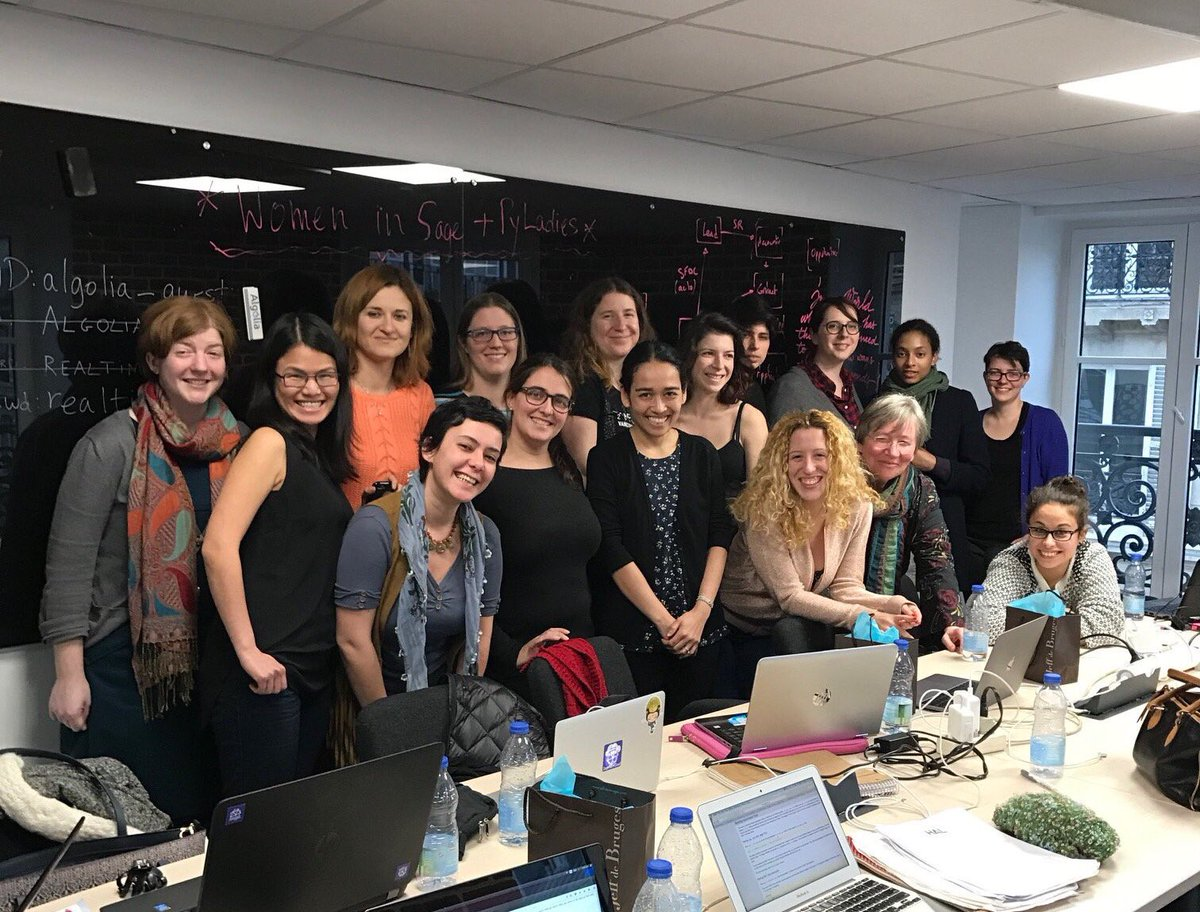
\includegraphics[scale=.2]{pyladies-WIS.jpg}
\caption*{The Women in Sage at the PyLadies coding afternoon}
\end{figure}



\end{event}

\begin{event}{Sage Days 93}{SageDays93}{Olot (ES),
2018-02-19 to 2018-03-04}{UB}{36}{1}{https://wiki.sagemath.org/days93}

\textbf{Main goals.}
The main goal of the Sage Days 93 were to
gather researcher specialists in Lie groups and advanced
SageMath and PARI/GP developers. The two goals were to implement
more Lie group theory in the softwares and conversely produce
experimental results for researchers.


\textbf{\ODK implication.}
%Describe how \ODK was involved and give a rough estimation of cost for \ODK

\ODK organizer: V. Delecroix.

\ODK provided the funding source for the workshop (accommodation,
subsistence and travel expenses) for about 20k\euro.

\textbf{Event summary.}
%Give a summary of your event

The Sage Days 93 took place in Olot (Spain) from february 19th to
march 4th. It was focused on the theory of Lie groups and their
subgroups.

There were 11 registered participants. A typical day of the workshop
consisted in talks and hacking session.

\textbf{Results and impact.}
% What did you achieve with this event? (If ever it impacted
% other \ODK tasks and deliverables, mention it here)
This was a development workshop dedicated to researcher in Lie groups
and their lattices. We obtain interesting feedback and developed
a lot of features related to Lie groups in SageMath and PARI/GP.
\end{event}


\begin{event}{Sage Days at Icerm}{SDIcerm}{ICERM Providence (United States), Jul. 23 -- 27, 2018}{PS}{78}{2}{https://icerm.brown.edu/topical_workshops/tw18-1-sage/}

\textbf{Main goals.} These Sage Days were focused on Combinatorics and Representation Theory. They were planned one week after the annual gathering of the algebraic combinatorics community at FPSAC 2018 (Hanover, New Hampshire).

\textbf{\ODK implication.} The event was not organized nor funded by \ODK. Nevertheless, it featured two talks by \ODK members (Nicolas Thiéry and Viviane Pons) and \ODK paid the travel expenses of some of the French participants.

\textbf{Event summary.} The event featured many presentations focusing on the link between \Sage development and research. It also allowed for some free coding time and discussions. Nicolas Thiéry and Viviane Pons both gave research presentations including some \Sage demo. It was an occasion to promote the \Sage docker and Jupyter live slides which is one of the use cases presented on \ODK website.

\textbf{Demographic.} Over 18 planed presentations, 9 were given by women.

\textbf{Results and impact.} This event was a good occasion for \ODK to connect the recent developments to the actual community and research. Beside \Sage development, many participants discovered docker during the event and showed lots of interest.

\end{event}




\subsection{Training activities for Sage in developing countries}

As open-source software developers, we wish our products
to be accessible to as many people as possible. Even though we offer
 a free access, there is still a technical gap in many 
developing countries that 
often prevents schools and researchers to benefit from our softwares.
This is why we believe the role of \ODK is to foster 
a wider community that does not leave a part of the world behind. In 
this section, we describe training activities that have been conducted 
through \ODK in this regard.

\begin{event}{6th Encuentro Colombiano de Combinatoria }{ECCO}{Barranquilla (Colombia), June 5 --- 16, 2018}{PS}{80}{1}{http://ecco2018.combinatoria.co/}

\textbf{Main goals.} ECCO (for \textit{Encuentro Colombiano de Combinatoria}) is a combinatorics research school organized every other year in Colombia. It gathered students from many countries (from both south-America and elsewhere) on advanced mathematics classes in an inclusive and welcoming environment. For the second time, it offered a \Sage class as well which goal is introduce \Sage to the students and help them develop their coding skills in relations to mathematics.

\textbf{ODK implication.} The \Sage class was given by Viviane Pons from ODK. Her travel costs were covered by ODK.

\textbf{Event summary.} Two afternoon sessions were organized (one for each week of the workshop). We had approximately 80 students on the first session and 40 on the second. Both sessions were organized in the computer room of the university so that all students would work whether they had material or not. Focus was given to introduction to \Sage in the context of combinatorics by offering many different tutorials and exercise worksheets for the students to choose from. We had created some specific worksheets in both English and Spanish directly related to the others courses of the conference so that the students could reproduce some of the results they had seen during classes and exercise sessions.

\textbf{Demographic.} We don't have access to the demographic information of the conference. Nevertheless we can say that most participants were students (from undergrad to PhD). Beside, this conference is in general very careful in creating a diverse and welcoming space.

\textbf{Results and impact.} This was the second time that we were at ECCO and we could see again that this was a great success. We had excellent feedbacks from both the students and the organizers. In 2016, the \Sage sessions were added late in the planning as extra sessions. In 2018, this is now an official \Sage course listed along the other mathematical classes of the conference. By being present twice in a row, we started a tradition of offering \Sage classes during this conference and this will be continued even after the end of ODK. For many students attending ECCO, the \Sage class is their first encounter with \Sage or even a mathematic software.

\begin{figure}[ht]
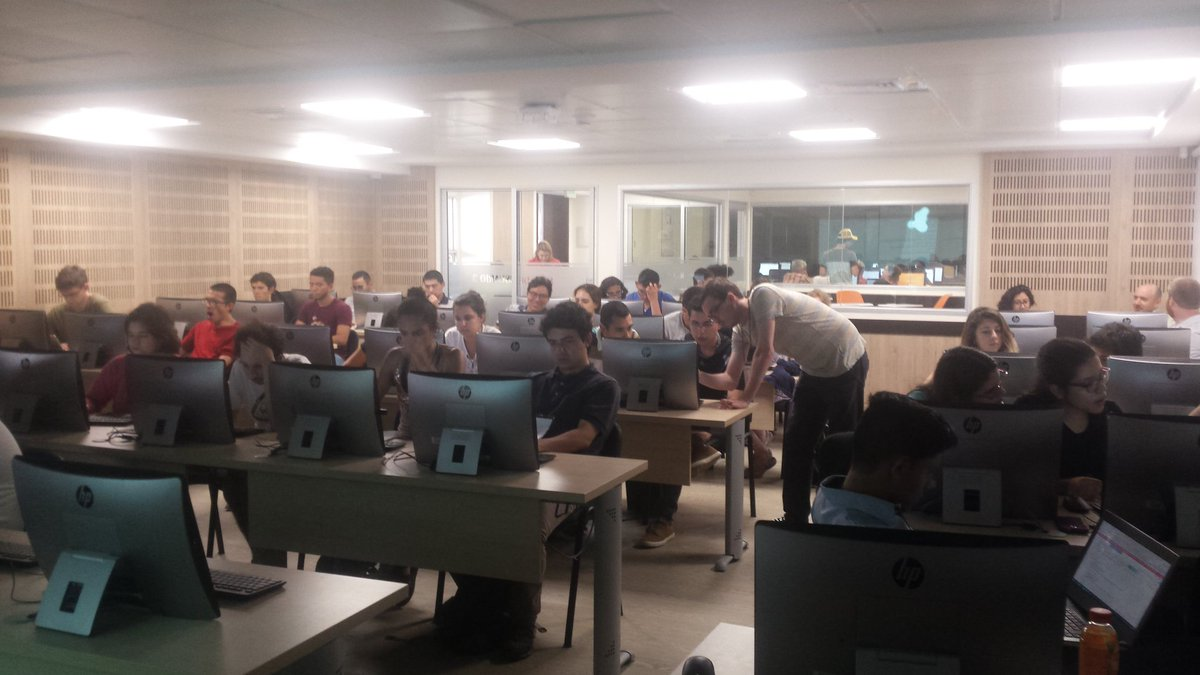
\includegraphics[scale=.2]{ECCO.jpg}
\caption*{Students working at ECCO}
\end{figure}



\end{event}


\subsection{Communication and participation to external events}

Dissemination activities also include the participation of \ODK
members to many different conferences of various size and topics
in computer science, mathematics, physics, and more. The goal is
to reach potential end-users, build bridges between communities and stay aware 
of current development in the scientific community.

We list here major events and communication. We have also put in place
a blog on our website: \url{http://opendreamkit.org/activities/} to track
these activities.

\begin{event}{Eurocomb 2017}{eurocomb}{Vienna, Aug. 28 -- Sept. 1st, 2017}{PS}{~20}{1}{http://www.dmg.tuwien.ac.at/eurocomb2017/}

\textbf{Main goals.} Eurocomb for \textit{European Conference on Combinatorics, Graph Theory and Applications} is one of the main international conferences on combinatorics. In 2017, it was organized in Vienna and gathered around 200 participants. This was a good occasion to present \Sage and \ODK to the community. We organized a small presentation which was included to the conference planing. Around 20 participants attended.

\textbf{\ODK implication.} Viviane Pons from \ODK was present at the conference and funded by \ODK.

\textbf{Event summary.} We gave a small presentation to introduce \Sage and \ODK to the participants. This included a demo on the CoCalc platform.

\textbf{Demographic.} Participants did not register specifically to the \Sage presentation, so we do not have any demographic information.

\textbf{Results and impact.} It is important that these short presentations happen regularly during main scientific events. Indeed, they keep the community up to date with current development. We received good feedback from the participants. It was an occasion for some of them to get introduced to \Sage for the first time and to open source math software in general.

\end{event}


\begin{event}{Netmath presentation}{netmath}{Kaiserslautern, Oct. 20, 2017}{PS}{5}{1}{https://www.netmath.de/}

\textbf{Main goals.} Presentation of \Sage, Jupyter and OpenDreamKit to the Netmath community.

\textbf{ODK implication.} Viviane from ODK did the presentation and the travel cost was covered by ODK.

\textbf{Event summary.} The Netmath community is an online network for university mathematic teaching, especially interested in sharing innovative methods and advice. This was their annual gathering and they invited us to present the project and how it can be used for teaching.

\textbf{Results and impact.} Some ODK tools such as \Sage and Jupyter can be very useful for teaching. Many ODK partners have worked into this direction and directly used some features developed by ODK and others for their teaching. This was an occasion to share our knowledge and expertise with another community. We received very good feedback from the Netmath organizers.


\end{event}


\section{Upcoming events and plans for the future}


\newpage\printbibliography

{\footnotesize All referenced ODK talks are available as annexes}

\end{document}

%%% Local Variables:
%%% mode: latex
%%% TeX-master: t
%%% End:
